\documentclass[sigconf,anonymous,review]{acmart}

\usepackage[normalem]{ulem}
\usepackage{amssymb}
\usepackage{amsmath}
\usepackage{algorithm} % environment for the algorithm code (like figure and table)
\usepackage{algorithmicx} % write the pseudo code
\usepackage[noend]{algpseudocode} % layout of the pseudo code
\usepackage{tikz} % needed for: tikz pics
\usepackage{xcolor}
\usepackage{xspace}
\usepackage{natbib}
\usepackage{graphicx}
\usepackage{subfigure}
%\usepackage[inline]{enumitem}

\newcommand{\TODO}[1]{{\bf \em \textcolor{red}{TODO: #1}\xspace}}

\newcommand{\todo}[2]{\textcolor{red}{$\bullet$ \textbf{Task:} #1; \textbf{Responsible:} #2}}

\newcommand{\sys}{VIPRE\xspace}
\newcommand{\sysfull}{Virtualized Intermittently-Powered Runtime Environment\xspace}

\setcopyright{rightsretained}

\acmDOI{http://dx.doi.org/xx.xxxx/xxxxxxx.xxxxxxx}

\acmISBN{978-1-xxxx-xxxx-x/17/11}

\acmConference[ASPLOS]{The 23rd ACM International Conference on Architectural Support for Programming Languages and Operating Systems}{March 24--28, 2017}{Williamsburg, VA, USA}

\acmYear{2017}

\copyrightyear{2017}

\acmPrice{15.00}

\begin{document}

\title[VIPRE: Virtualized Intermittently-Powered Runtime Environment]{VIPRE: Virtualized Intermittently-Powered Runtime Environment}

%Note: order of authors placed randomly

\author{Kiwan Maeng}
%\authornote{}
%\orcid{}
\affiliation{%
	\institution{Carnegie Mellon University}
	\streetaddress{4720 Forbes Avenue}
	\city{Pittsburgh} 
	\state{PA} 
	\postcode{15213}
}
\email{kmaeng@andrew.cmu.edu}

\author{Alexei Colin}
%\authornote{}
%\orcid{}
\affiliation{%
	\institution{Carnegie Mellon University}
	\streetaddress{4720 Forbes Avenue}
	\city{Pittsburgh} 
	\state{PA} 
	\postcode{15213}
}
\email{acolin@andrew.cmu.edu}

\author{Brandon Lucia}
%\authornote{}
%\orcid{}
\affiliation{%
	\institution{Carnegie Mellon University}
	\streetaddress{4720 Forbes Avenue}
	\city{Pittsburgh} 
	\state{PA} 
	\postcode{15213}
}
\email{blucia@andrew.cmu.edu}

\author{Amjad Yousef Majid}
%\authornote{}
%\orcid{}
\affiliation{%
	\institution{Delft University of Technology}
	\streetaddress{Mekelweg 4}
	\city{Delft, The Netherlands} 
	\state{Zuid Holland} 
	\postcode{2628\,CD}
}
\email{a.y.majid@tudelft.nl}

\author{Kas{\i}m Sinan Y{\i}ld{\i}r{\i}m}
%\authornote{}
%\orcid{}
\affiliation{%
	\institution{Delft University of Technology}
	\streetaddress{Mekelweg 4}
	\city{Delft, The Netherlands} 
	\state{Zuid Holland} 
	\postcode{2628\,CD}
}
\email{k.s.yildirim@tudelft.nl}

\author{Przemys{\l}aw Pawe{\l}czak}
%\authornote{}
%\orcid{}
\affiliation{%
	\institution{Delft University of Technology}
	\streetaddress{Mekelweg 4}
	\city{Delft, The Netherlands} 
	\state{Zuid Holland} 
	\postcode{2628\,CD}
}
\email{p.pawelczak@tudelft.nl}

\renewcommand{\shortauthors}{A. Y. Majid et al.}

\begin{abstract}
% Connecting the work to a real-world problem
Embedded devices in the Internet of Things (IoT) gain new deployment
opportunities when their hardware is free of batteries and powered by ambient
energy.
% The main problem that we are tackling
Energy harvested from the environment, however, is unpredictable
and can only power a device intermittently.
% The already proposed solution to the main problem
In the intermittent execution model, computation is frequently interrupted by
power failures, and to make forward progress, the system must save intermediate
program state into non-volatile memory.

% The problem of the proposed solutions 
Task-based programming models that execute at the granularity of
statically-defined tasks, offer an efficient alternative to checkpointing.
%
Existing task-based systems, however, fix their task size at compile time and
operate without any regard to the changing energy conditions at runtime.
%
When tasks are sized without accounting for available energy, state may be
persisted either more frequently than unnecessary or not frequently enough for
the program to make progress and terminate.
%
% Our main claim 
To address this challenge, we propose Coala, an \emph{adaptive} task-based
execution model that colesces or downscales static tasks at runtime in response
to changing energy availability.
% show off
% main benefits of Coala
Coala ensures that power failures cannot leave the program state in
non-volatile memory inconsistent using a specialized memory virtualization
mechanism.
%
Our evaluation on a real energy-harvesting device demonstrates the benefits of
adaptive task coalescing and downscaling, and highlights Coala's performance
improvements over a state-of-art task-based system.



\end{abstract}

% The code below should be generated by the tool at 
%http://dl.acm.org/ccs.cfm Please copy and paste the code instead of the 
%example below. 

\begin{CCSXML}
	<ccs2012>
	<concept>
	<concept_id>10010520.10010553.10010562.10010564</concept_id>
	<concept_desc>Computer systems organization~Embedded 
	software</concept_desc>
	<concept_significance>500</concept_significance>
	</concept>
	<concept>
	<concept_id>10010520.10010575.10010578</concept_id>
	<concept_desc>Computer systems organization~Availability</concept_desc>
	<concept_significance>300</concept_significance>
	</concept>
	<concept>
	<concept_id>10011007.10010940.10010941.10010949.10010957.10010688</concept_id>
	<concept_desc>Software and its engineering~Scheduling</concept_desc>
	<concept_significance>300</concept_significance>
	</concept>
	<concept>
	<concept_id>10011007.10010940.10010941.10010949.10010965</concept_id>
	<concept_desc>Software and its engineering~Communications 
	management</concept_desc>
	<concept_significance>300</concept_significance>
	</concept>
	<concept>
	<concept_id>10011007.10010940.10010971.10010564</concept_id>
	<concept_desc>Software and its engineering~Embedded 
	software</concept_desc>
	<concept_significance>300</concept_significance>
	</concept>
	</ccs2012>
\end{CCSXML}

\ccsdesc[500]{Computer systems organization~Embedded software}
\ccsdesc[300]{Computer systems organization~Availability}
\ccsdesc[300]{Software and its engineering~Scheduling}
\ccsdesc[300]{Software and its engineering~Communications management}
\ccsdesc[300]{Software and its engineering~Embedded software}

\keywords{Energy harvesting, transient operation, operating system}

\maketitle

\section{Introduction}
\label{sec:intro}

%\TODO{VIPER: Virtualised Intermittent Programming model, Execution model, and Runtime environment}
%\TODO{PREVIEW: Programming and Runtime Environment with Virtualised Intermittent Execution Windows}

Advances in processor efficiency along with the development of energy-harvesting systems have created a new category of devices that require neither a battery nor a tethered power supply~\cite{prasad_comst_2014,lucia_snapl_2017,soyata_csm_2016}. These devices operate using ambient energy, such as radio frequency transmissions~\cite{rf_powered_computing_gollakota_2014},
light~\cite{margolies_infocom_2016,margolies_tosn_2016}, and vibration~\cite{gorlatova_sigmetrics_2014}. Incorporating compute, storage, sensing, and communication hardware~\cite{wisp5,moo,capybara}, such devices are a promising technology for use in the Internet of Things~\cite{ku_cst_2016}, in-body~\cite{nadeau_naturebio_2017} and on-body~\cite{bandodkar_electroanalysis_2015} medical systems, and energy-harvesting nano-satellites~\cite{kicksat,capybara}. Energy-harvesting devices create unique challenges because they operate {\em intermittently} when energy is available~\cite{hicks_isca_2017,lucia_snapl_2017}. An energy-harvesting device buffers energy in a small storage capacitor~\cite{gorlatova_tmc_2013,gunduz_commag_2014} and operates when a threshold amount of energy has accumulated. Harvestable energy sources are low-power (e.g., \si{\nano\watt}\ to \si{\micro\watt}) compared to a platform's operating power level (hundreds of \si{\micro\watt}\ to \si{\milli\watt}). A device operates briefly until it depletes its buffered energy, after which, it shuts down and recharges to operate again later---corresponding to the {\em intermittent execution model}~\cite{dino,lucia_snapl_2017} composed of operation---power failure---restart cycles. The recharge and discharge intervals---which correspond to the device's inactive and active time---vary depending on the underlying hardware, such as the size of the energy buffering~\cite{capybara}, and energy conditions. For example, some devices discharge and restart $\approx$10 to $\approx$100 times per second~\cite{tan_infocom_2016,mementos,nvp}.

Upon power failures, a device loses the volatile state in its registers, stack, SRAM, and retains the state of any non-volatile memory, such as FRAM. While capturing periodic checkpoints~\cite{mementos,quickrecall} and sleep scheduling~\cite{dewdrop,hibernus,hibernusplusplus} help preserve execution progress, failures can leave non-volatile state incorrect, partially updated. These inconsistencies cause intermittent execution to deviate from continuously-powered behavior, often leading to an unrecoverable application failure~\cite{dino,edb}. Prior work developed two main approaches to deal with data inconsistency for intermittently-powered devices: (i) \emph{software-based programming and execution models}~\cite{dino,ratchet,chain,alpaca} and (ii) \emph{hardware-based computer architecture support}~\cite{hicks_isca_2017,idetic,nvp}. Complex hardware architectural changes are expensive to design, verify, and manufacture. New hardware architectures are also inapplicable to existing systems~\cite{hicks_isca_2017,nvp}. Software approaches are simpler and applicable to existing devices today. Therefore, this work focuses on software approaches. In particular we address the key limitation of task-based programming and execution model, that is the {\em inflexibility} and \emph{energy-unawareness} of statically decomposing a program into tasks.
%
\begin{figure}
    \centering
    \includegraphics[width=\columnwidth]{figures/intro-figure.pdf}
    \caption{Task coalescing at runtime reduces time and energy overhead in task-based intermittent programming models by performing fewer commits (denoted as \texttt{C}) of individual tasks (denoted as \texttt{Tx}). On the other hand, task splitting reduces wasted computation and enables termination for bigger tasks.}
    \label{fig:coalesce}
\end{figure}

%\textbf{Task Decomposition of Intermittent Programs.} 

\textbf{Crucial Drawback of Static Task Decomposition.} Task-based programming and execution models require a programmer~\cite{alpaca,chain} or a compiler~\cite{baghsorkhi_cgo_2018} to statically decompose a program into a collection of tasks. A \emph{task}, a top level function, can include arbitrary computation that should be executed despite arbitrarily-timed power failures. The programmer (or a compiler) explicitly expresses task-to-task control flow. Fig.~\ref{fig:coalesce} (left) illustrates how a program's tasks execute and shows how tasks transitions can impose a runtime overhead. At each transition, the system incurs an overhead to track and atomically commit modifications to the non-volatile memory, to maintain consistency of program state~\cite{chain,alpaca}. The more task transitions a program requires, the more commit overhead is incurred by the system at runtime. A programmer may thus create very large tasks in an attempt to reduce task transitions overhead. However, a large task may require more energy to complete than a device's fixed hardware energy buffer can hold, which may lead to a task \emph{non-termination} problem (see Fig.~\ref{fig:coalesce}(right)). To eliminate this risk, existing systems require the programmer to decompose a program into small tasks to preserve execution progress. These constraints on task sizing lead to the following \emph{dilemma}: should large tasks be used, that are efficient but risk non-termination, or small tasks that are guaranteed to complete but incur a high task transition and commit overhead?

\textbf{Challenges and Contributions.} We introduce \sys: a new task-based system that employs \emph{adaptive task size execution by task coalescing and splitting}. By means of this novel technique, small tasks can be executed efficiently by trimming unnecessary overheads \emph{dynamically}, meanwhile avoiding the risk of non-termination. \sys accepts any static decomposition and it coalesces (groups) tasks or splits them (see again Fig.~\ref{fig:coalesce}) based on the estimated energy availability without demanding any hardware support. To the best of our knowledge, \sys is the only system that guarantees forward progress for any statically-defined tasks or energy storage sizes. 

The unique contributions of \sys in relation to challenges of task-based systems revealed by this work are as follows:

\begin{itemize}

\item[C1] \emph{Overcoming Task Transition Overhead:} given unpredictable incoming energy, how to save computation state at task transitions as rare as possible? \sys tries to minimize task transition overhead by estimating energy conditions at run-time using \emph{recent execution history} as a metric.

\item[C2] \emph{Dynamic Memory Consistency Handling:} merging static tasks on the fly rises  the need for dynamic memory consistency handling. This leads to the second challenge: how to dynamically detect inter-coalesced-task data dependencies and ensure efficient protection against power interrupts? \sys addresses this challenge by using a novel approach called \emph{dynamic group privatization}---performing real-time dependency tracking to enable protection on a task transition. Individual variables tracking, however, slows down a system dramatically. Therefore, \sys keeps memory consistent through \emph{memory virtualization} optimized for bulk accesses to task-shared data with high locality.

%Therefore, \sys protects global variables in a batch. Moreover, it optimizes data transfers by using Direct Memory Access (DMA).

\item[C3] \emph{Ensuring Task Termination:} a static task decomposition model assumes that each task can execute to completion. If the hardware energy buffer provides inadequate energy to execute each task to completion, a program will not terminate~\cite{cleancut_2018}. This leads to a third challenge: how to enable the dynamic execution model to progress on a sub-task level? To avoid non-termination under adverse energy conditions, \sys uses a novel timer-based {\em partial task commit} mechanism, inspired by~\cite{ratchet}. Partial execution avoids non-termination by committing the intermediate state of a long-running task that has repeatedly failed and restarted.

\end{itemize}

To asses the benefits of \sys over existing task-based systems, we implemented and tested six benchmarks on a real energy-harvesting platform. Our evaluation not only shows that \sys reduces run time by up to 54\%, and by 26\% on average, but also is able to continue the execution where static task-based systems fail.
 
The rest of this paper is organized as follows. Section~\ref{sec:background} provides background on intermittent computing.
Section~\ref{sec:systemdescription} provides an overview of \sys, while Section~\ref{sec:task_adaptation} describes \sys's task adaptation mechanism. The dynamic group privatization is explained in Section~\ref{sec:memory_virtulaization}. Implementation details of \sys are given in Section~\ref{sec:implementation}. Sections~\ref{sec:methodology} and~\ref{sec:evaluation} describe \sys's evaluation methodology and results. Section~\ref{sec:related_work} positions \sys in the context of related work and Section~\ref{sec:conclusions} concludes and discusses future work.

\section{Computation on Intermittent Devices: Background}
\label{sec:background}

Performing complex operations on battery-less energy harvesting embedded platforms is challenging from many points of view. Here we shall briefly provide a background on computation with energy harvesting embedded systems. 

\subsection{Energy Harvesting: Background}

Supplying power to tiny embedded computers using batteries alone is not sustainable. Batteries are a great pollutant. A solution is to replace batteries with smaller, but more environment friendly capacitors and supply power directly from the ambient energy sources. 

What platforms enable intermittent computation: WISP~\cite{} (with its variants such as WISPCam~\cite{}), Moo~\cite{}, ambient backscatter~\cite{}, or computation RFID commercial platforms such as~\cite{}. In case of the above platforms, the main source of energy is electromagnetic radiation in the radio frequency range.

Application include long-term battery-less monitoring. One example is the distributed monitoring of moisture of large plant fields during vegetation~\cite{}. Other applications include battery-less image capture and processing~\cite{}, distributed low-power networking~\cite{}.

Energy provided from the ambient is not stable and difficult to predict accurately. Combined with the fact that energy supply is small, there is little leeway to store enough of energy to guarantee prolonged periods of computation. Energy breaks happen every hundred of ms~\cite{}.

Solution to the problem is to divide the program into smaller pieces that guarantee execution within a discharge region and track the state of the program in-between the program part execution times. 

\subsection{(Task-based) Intermittent Computing: Background}

\begin{figure}
	\centering
	%\includegraphics[width=0.25\columnwidth]{figures/}
	\caption{Two problems with fixed-size task in intermittent execution. (a) task underestimation: task executed at device with capacitor size $X$, will not execute at device with capacitor $X\gg Y$; (b) task overestimation: with stable energy source task tracking causes unnecessary overhead.}
	\label{fig:fixed_task_problem}
\end{figure}

Various capacitor sizes of intermittent device result in a program being executed 

Other forms of intermittent platforms will share the same problem. One of them considers actuation platforms, which will be powered directly from energy harvesting sources~\cite{}. will share the energy storage with computing platform. However, power supply for actuators is order of magnitude larger than for computation. Therefore, although capacitor is large enough to perform computation alone, energy to power actuators takes precedence leaving not much space for computing.


\TODO{Elaborate on the ``key challenge'' paragraphs near the end of the intro.}

\section{\sysfull}
\label{sec:overeall_system}

\begin{figure}
	\centering
	%\includegraphics[width=0.25\columnwidth]{figures/}
	\caption{\sys top-level description.}
	\label{fig:}
\end{figure}

Describe the overall system, the programming model, and the semantics/execution model. This should include a discussion of memory virtualization and task coalescing.

\section{Memory Virtualization}
\label{sec:memory_virtulaization}

\begin{figure}
	\centering
	%\includegraphics[width=0.25\columnwidth]{figures/}
	\caption{Memory virtualization architecture.}
	\label{fig:}
\end{figure}

\section{Task Coalescing}
\label{sec:memory_virtulaization}

\begin{figure}
	\centering
	%\includegraphics[width=0.25\columnwidth]{figures/}
	\caption{Task coalescing architecture.}
	\label{fig:}
\end{figure}

\section{Discussion}
\label{sec:discussion}

\section{Methodology and Evaluation}
\label{sec:methodology_evaluation}

\section{Related Work}
\label{sec:related_work}

\section{Conclusions}
\label{sec:conclusions}

This paper presented \sys: \sysfull.

%%%%%

\section{Old Introduction}
	Intermittently powered devices (IPDs) are battery-less devices that utilize the ambient energy to sense, compute and, communicate. For example, Wireless Identification and Sensing platform WISP \cite{wisp} uses the RF signal power to drive its computation and communication. Because of the reliance of TPDs on intermittent power supply, the harvested energy when it is available, their programs are susceptible to a very frequent power interrupts, in the order of tens of millisconds~\cite{}. Therefore, these devices require a different software execution model that complies with the nature of a discontinuous power supply. 

	The intermittent (discontinuous) execution model defines a program execution as cumulative discrete process. The main difference between the intermittent and the conventional (or continuous) execution models is that, a power failure is seen by the continuous model as an \emph{exception} that may reset the progress of a program to its beginning. Whereas, in intermittent execution a power failure is regarded as a temporary \emph{pause} to the execution that may result in some progress degradation. Generally we can classify the intermittent execution model into: 
	\begin{itemize}
		\item \emph{Sequential Execution Model}:
			Under this model a program is seen as one big idempotent operational region that has one common context. Generally, The progress of the program is saved and updated by means of checkpointing---where all the program context (e.g. CPU registers, the stack and the global variables) is saved to a non-volatile memory. Normally, the sequential model relies on a hardware assistant to measure the voltage level in the energy reservoir to place a checkpoint~\cite{mementos, harvOS, hibernus}. The benefit of this model is that it does not require code modification by a programmer. However, it has a number of drawbacks: (i) It suffers from significant overhead \cite{chain}; (ii) the programmer should not access the non-volatile memory to guarantee the consistency of the memory~\cite{xxxx}; and (iii) it restricts the IPDs to run only a single application~\cite{inos}. 
		\item \emph{Modular Intermittent Execution Model}:
			At the heart of this model is the concept of an idempotent task. The idempotent task is C function that does not have arguments and does not return a value. This task uses a well defined interface to interact with the non-volatile memory. Therefore, it tolerates arbitrary number of power interrupts. This model, generally, produces less overhead~\cite{chain} and allows multiple applications to run on an IPD by interleaving their tasks~\cite{inos}. However, it obviously requires code modification---for example, if an algorithm is written according to the continuous execution model it has to be splitted, by a programmer, into small tasks to run under the modular intermittent execution model.
	\end{itemize}

Despite that the superiority of the Modular Intermittent Execution model, it is still a static approach that completely depends on a programmer's estimation which is mostly result in a sub-optimal code devision. Moreover, this model can only consider a single hardware configuration and it does not take environment changing into considerations. 




% Energy source


% The intermittent execution is cumulative discrete process. The intermittent execution model is only able to execute a few number of instructions, as compared to the conventional (continuous) model, before its progress is terminated. Therefore, the intermittent execution model adapts an execution progress state saving mechanism. This mechanism is realized either by means of a checkpoint~\cite{}, where all the context of the program is saved into non-volatile memory. Or 

% This progress state saving mechanism is normally injected into a program either by a compiler~\cite{}. A compiler injects trigger pointers to checkpoint (save) the context of the program into the non-volatile memory.  or it is added by a programmer~\cite{chain}. [compare these two approaches]...

% We define virtualization within the context of intermittent execution as utilizing the volatile memory instead of non-volatile when the intermittent execution model attempts to access the non-volatile memory. 

\subsection{Why not Adapting Current Approaches}
Here we highlight the challenges of adapting the state-of-the-art proposed methods to enable the execution of dynamic task sizes. 
%
%	\begin{figure}[t]
%	    \centering
%	         \subfigure[Chain: Sequential task execution flow control.]{\includegraphics[width=0.35\columnwidth]{figures/dynamic-chain.pdf} \label{fig:DynamicChainSeq} } 
%	         \subfigure[Chain: Random task execution flow control.]{\includegraphics[width=0.61\columnwidth]{figures/dynamic-chain-2.pdf} \label{fig:DynamicChainRan}}
%	    \caption{Task flow control of Chain}
%	    \label{fig:DynamicChain}
%	\end{figure}


\noindent\textbf{Chain: Tasks and Channels for Reliable Intermittent Programs } \\
Some of the main problems in modifying Chain to support dynamic task's size are:

\begin{itemize}
	\item \emph{Multi-versioning system:} Chain defines for each task its own input that is not shared with other tasks. This design decision makes the benefit of merging tasks of less importance since each task is interacting with its own variables. 
	\item \emph{Direct FRAM system:} Chain tasks directly access FRAM which is more energy expensive Than SRAM. As result of being multi-versioning system that directly interacts with FRAM, Chain has a significant energy consumption overhead. 
	\item \emph{Irreversible tasks transitions:} According to the Chain programming model, each task calls the next one. The transition is done through functions calls and manually clearing the stack, to prevent the stack overflow problem. This approach make all the transitions firm ones which prevent task merging.
	\item \emph{All channels are required:} Fig.~\ref{fig:DynamicChainSeq} shows that if the task control flow is a circular with no branches then task merging is possible. Moreover, all the intra-merged-tasks channel can be committed to SRAM instead of FRAM to save energy. However, this execution path is only a special. If the general case (see Fig.~\ref{fig:DynamicChainRan}) is considered then leaving out the intra-merged-task channels might result in data inconsistency---If an application tries to access a merged task from the middle after a power interrupt then the input for that task is not ready which result in an incorrect execution. 


\end{itemize}


\noindent\textbf{Alpaca: Intermittent Execution without Checkpoints} \\
Some of the main problems in modifying Alpaca to support dynamic task's size are:

\begin{itemize}
	\item \emph{Privatization:} The core concept of Alpaca is privatization. Privatization depends completely on detecting the variables that have a Write-after-read dependency within the scope of a task. Therefore, if tasks are on-demand merged the scope of these dependencies are changed and the static analysis to privatize these variables is not valid anymore and data consistency can not be preserved.  

	\item \emph{Irreversible tasks transitions:} Similar to Chain problem. 

\end{itemize}

\noindent\textbf{Virtualizing Modular Intermittent Execution Model}

		An Intermittently executed program, as seen by the modular intermittent execution model, is a chain of tasks with a firm transition from one to another. 
		Virtualizing this model means softening a number of transitions, by keeping the state of the execution progress in the volatile memory, to construct a bigger \emph{virtual task} to reduce energy consumption. Ideally, the size of the virtual task should match the length of a continuous interval of the intermittent power supply for the best performance. Another form of virtualization can be achieved by reducing the number of non-volatile memory accesses. This can be done by having a temporary copy of a global variable in the volatile memory (similar to the catching principle) and a task interacts with it and updates it before writing back the most recent value to the non-volatile memory during the commit process.

		In this paper we are introducing VIPOS a runtime library the implement the Virtualed Intermittent Execution Model. VIPOS adapts two methods for data protection. One relies on a virtual buffer and the other uses the Direct Memory Access (DMA). VIPOS is able to approach the optimal tasks devision during the runtime. VIPOS reduces an application execution time by XX and the energy by XX. 


\subsection{Contributions}
	 \begin{enumerate}
		 \item We have developed an algorithm that is able to determine the size of a virtual task based on the history of the execution of an application. 
		 \item We enable efficient code portability by requiring that a real task to small and merging them during the execution.   
	\end{enumerate}


 \section{Preliminary Results}
 \label{sec:prelResults}

\begin{figure}[t]
    \centering
         \subfigure[The energy cost of FRAM/SRAM \textbf{writes} operations.]{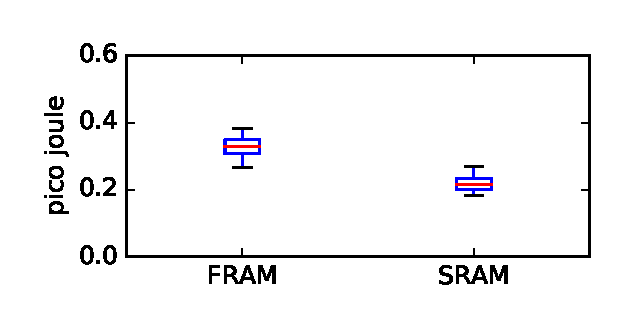
\includegraphics[width=0.48\columnwidth]{figures/fram_write.eps} }
         \subfigure[The energy cost of FRAM/SRAM \textbf{read} operations.]{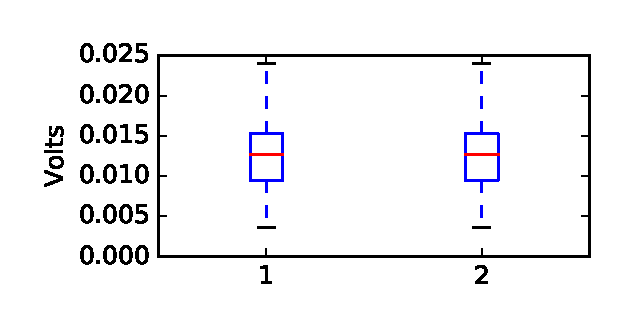
\includegraphics[width=0.48\columnwidth]{figures/fram_read.eps}}
    \caption{The energy cost of accessing volatile/non-volatile memory}
    \label{fig:framEnergy}
\end{figure}

Since the Intermittent execution models rely on the non-volatile memory to enable long-running operation, it is important to characterize the energy consumption of accessing this type of memory as compare to the volatile one.

Four applications are developed to measure the energy consumption of \emph{Accessing} the FRAM and SRAM of the MSP430FR5969 microcontroller~\cite{xxx}. The interference free debugger (EDB)~\cite{xxx} is used as the energy measurement tool. The EDB probes the energy buffer before and after accessing the FRAM/SRAM 1600 times, This large number of FRAM access is used to increase the reliability of the results generated by the used measurement tool (e.g. reducing the effect of the quantization error).  The energy buffer is charged, using the EDB, to $\approx$ 2.45 volts \textbf{only} at the beginning of the execution and of the programs. The write operations were performed by writing literal values, random numbers, to the memory. However, a read operation must be followed by a write operation, therefore, we chose to write a read value to SRAM. Fig.~\ref{fig:framEnergy} shows that an FRAM access equals $\frac{3}{2}$ SRAM access~\footnote{We would like to mentioned that TI has already mentioned in this document~\cite{xxxx} that FRAM write access is more energy expensive than SRAM write access. However, TI does not quantify the energy overhead.}. Therefore, reducing FRAM access is desirable when developing  energy limited software solution  




\section{VIPOS: Virtualized Intermittently Powered Runtime Environment}
VIPOS is runtime library that facilitates tasks navigation and preserves data/memory consistency of the IPDs. It is able, on-demand, to merge tasks to reduce the number of commits to the non-volatile memory.

\section{\sys: Data/Memory Protection Methods}

\begin{figure}[t]
	\centering
	\includegraphics[width=0.8\columnwidth]{figures/iposCommitSize}
	\caption{...}
	\label{fig:virtOperationalBuf}
\end{figure}


\sys data consistency preservation methods are designed with goal of minimal interaction between the CPU and FRAM to reduce energy consumption (see Section~\ref{sec:prelResults}). These data/memory protection methods enables \sys to tolerate arbitrary number of power failures. 

	\subsubsection{Virtualized Operational Buffer}

		\begin{algorithm}[t]
			\caption{Virtualized Operational Buffer}
			\label{algo:virtuBufWrite}
			\scriptsize
			%\small
			\begin{algorithmic}[1]
				\State $var \in \text{\{global variables\}} $ 
				\State \label{lst:virtuBufWrite:line:begin}\Call{Virtual Task()}{} 
				\While { \textit{executing} } \Comment{Execution stage}
					\State $var$  $\rightarrow$ \textsf{volatile buffer} \label{lst:virtuBufWrite:line:output}
					\If { $var$  in \textsf{ volatile buffer} }				\label{lst:virtuBufWrite:line:inputBegin}
							\State $var$  $\leftarrow$  \textsf{volatile buffer} 
						\Else 
							\State $var$  $\leftarrow$  \textsf{FRAM}		\label{lst:virtuBufWrite:line:inputEnd}
						\EndIf

					\If {power interrupts}
						\State back to \ref{lst:virtuBufWrite:line:begin}
					\EndIf
				\EndWhile

				\While{  $\textsf{volatile buffer}\not=\emptyset$  } \label{lst:virtuBufWrite:line:commitBegin} \Comment{ First phase commit}
					\State \textsf{volatile buffer} $\rightarrow$  \textsf{persistent buffer}
					\If {power interrupts}
						\State discard \textsf{persistent buffer}
						\State back to  \ref{lst:virtuBufWrite:line:begin} 
						\State   \label{lst:virtuBufWrite:line:commitEnd}
					\EndIf
				\EndWhile 

				\While{ $\textsf{persistent buffer}\not=\emptyset$ } \label{lst:virtuBufWrite:line:SecCommitBegin} \Comment{Second phase commit}
					\State \textsf{persistent buffer} $\rightarrow$ FRAM 
					\If {power interrupts}
						\State Continue
					\EndIf
				\EndWhile 
				\State     \label{lst:virtuBufWrite:line:SecCommitEnd}
				\State return
			\end{algorithmic}
		\end{algorithm}


		Since accessing FRAM is more energy expensive and slower than accessing SRAM, preventing frequent access to FRAM (i.e. during looping operations) is desirable. Therefore, the first proposed protection method utilizes a volatile buffer that holds temporary all the outputs of a virtual task (see Algorithm~\ref{algo:virtuBufWrite} line~\ref{lst:virtuBufWrite:line:output}). Consequently, a virtual task must first attempt to read a global variable from the volatile buffer before trying to obtain the value from the non-volatile memory (see Algorithm~\ref{algo:virtuBufWrite} lines~\ref{lst:virtuBufWrite:line:inputBegin}-\ref{lst:virtuBufWrite:line:inputEnd}) to ensure a correct execution progress and the consistency of the memory. Once the execution of a virtual task is done, the first phase of the commit process is started by copying the volatile buffer to a persistent buffer (see Algorithm~\ref{algo:virtuBufWrite} lines~\ref{lst:virtuBufWrite:line:commitBegin}-\ref{lst:virtuBufWrite:line:commitEnd}). If the power is interrupted the persistent buffer must be discarded and the execution must start again from the beginning of the virtual task. In another words, the first phase commit must be performed atomically to preserve the consistency of the output of a virtual task. The second phase commit is a power failure immune precess that is responsible for distributing the global variables to their final locations and make the non-volatile memory consistent and synchronized with the computation progress (see Algorithm~\ref{algo:virtuBufWrite}lines~\ref{lst:virtuBufWrite:line:SecCommitBegin}-\ref{lst:virtuBufWrite:line:SecCommitEnd}).


	\paragraph{Virtualized Operational Buffer: Implementation} 

		We implement a reference implementation of \sys that uses virtualized Operational buffer to protect the data against power failure. 
		\paragraph{Virtual Buffer}
			We realized the virtaulzed buffer as a volatile hashed table of linked lists. The hashing technique was chosen to reduce the buffer searching time and the linked lists are used to prevent data loss when there is a conflict between multiple variables---If two variables have the same hash value they will occupy the same cell, however, with linked list a new node will be created for each variable to resolve the conflict and protect the data. The hashing function is based on the observation that the virtual addresses of the memory cells have approximately a flat distribution over the memory addressing space and the fact that each entry, of the virtual table, has the address and the value of a variable. As such, by using the least significant bits as an index to access the virtual buffer the hash function distributes its inputs uniformly in the virtual buffer. Accordingly, the linked lists search time, on average, is reduced. 

			Despite the fact that the linked lists reduce the average complexity of searching the virtual buffer significantly, they introduce a number of drawbacks: (i) the linked list data structure introduce a non-negligible memory overhead while it relies on a limited memory section, namely the heap; (ii) traversing the linked list is relatively slow. Therefore, we re-implemented the virtual buffer, after observing that most of the global variables have the same most significant bits, as a bigger hashed table that does not allow entries conflict. To eliminate the need for searching the hashed table linearly while committing its entries, we add a new buffer that holds the indices of the occupied cells of the hashed table. This table is of the same length as the hashed table. We can reason about the benefit of this buffer as follows: if we assume that the global variables are evenly divided between the tasks, then this buffer reduces the commit time by a factor equal to the number of tasks.   

		\paragraph{Persistent Buffer}
			The persistent buffer is implemented as static array of tuples, where each tuple holds  the address and the value of a variable. This data structure is very suitable for the second phase commit where each element has to be committed to its finial location. However, the complexity of committing this buffer is of size $O(N)$, where $N$ equals the length of the buffer. Therefore, the size of the buffer can have dramatic effect on the performance of \sys---On one hand, if the size of the buffer is small the buffer overflow problem will be very serious. On the other hand, if the size of the buffer is large \sys will experience a significant performance degradation. However, by observing the type of the information that this buffer holds, namely memory addresses, we can, on average, reduce the complexity of committing this buffer by defining the \emph{effective size} of the buffer to be the size of the buffer up to the first cell that holds an invalid memory address. Moreover, since this buffer is in FRAM which is much bigger than SRAM its size can be relatively big. 

		% \paragraph{Virtualized Operational Buffer: delay analysis}[initial results]

		% \begin{figure}[t]
		% 	\centering
		% 	\includegraphics[width=\columnwidth]{figures/virtual_buffer_size.eps}
		% 	\caption{\sys based on virtualized Operational Buffer. It runs the decompression application with different buffer configurarions. EPB: Enhanced Persistent Buffer. NR: no read operation from the buffer. NRW: not read or write operations from the buffer.}
		% 	\label{fig:virtOperationalBuf}
		% \end{figure}

		% 	To analyze the performance of \sys versus the sizes of the virtual buffer and the persistent buffer we setup the following experiment. We let IPOS to run the decompression application---until the data decompression is completely finished---and we capture the execution time using a logic analyzer~\cite{xxx}. The results presented in Fig.~\ref{fig:virtOperationalBuf} show the \sys has its best performance when the virtual buffer size is 16, where the execution time was $\approx$196 ms. 

		% 	All the experiments were done with a persistent buffer of size 100. However, the bar labeled with "EPB/16" in  Fig.~\ref{fig:virtOperationalBuf} shows the effect of the enhanced commit process that uses the buffer effective size instead of the buffer maximum size. We see that the execution time is reduced to $\approx$80 ms. Furthermore, we quantized the overhead of the read operations from the buffer, by eliminating this operation, and the bar labeled with "NR" shows that it cost  $\approx$10 ms. Moreover, the overhead of the read and write operations is $\approx$34 ms as compared to \sys best performance, see the bar labeled with "NRW" in Fig.~\ref{fig:virtOperationalBuf}. 


\subsubsection{ Direct Memory Access Based Protection Method (better name is needed)}
%
	\begin{figure}[t]
		\centering
         \subfloat[The time needed to transfer a block of data using pointers versus Direct Memory Access (DMA).]{\includegraphics[width=0.48\columnwidth]{figures/dmaSize_time.eps} }
	     \subfloat[The energy needed to transfer a block of data using pointers versus Direct Memory Access (DMA).]{\includegraphics[width=0.48\columnwidth]{figures/energyConsumptionDMA_SW.eps}}
		\caption{Time and energy consumption of moving a block of data from SRAM to FRAM}
		\label{fig:dmaTimeEnergy}
	\end{figure}
%
	Since accessing/updating buffers is more costly than directly accessing FRAM, at least without specialized hardware~\cite{clank}, we introduce the second method to apply the virtualization principle to the Modular Execution Model. This method utilizing the Direct Memory Access (DMA) Module. As Fig.~\ref{fig:dmaTimeEnergy} shows that DMA is much more efficient in transferring a block of data than the conventional (pointer based) way from the energy and time perspectives. 

	This method combines a number of techniques to preserve the persistence and consistency of the data. It backs up the status of the global variables in the non-volatile memory, and double buffers them to guarantee their consistency. Furthermore, on each power up it populates the global variables in the volatile memory from the most recent back up in the non-volatile memory to enable a faster task execution since the task does not need to interact with non-volatile memory which is generally slower and more energy expensive.   



\subsection{VIPOS: The Virtualizing Engine}
\subsubsection{Power Interrupt Immune Scheduler}
It utilizes a persistent circular buffer (persistent linked-list) to keep the state of a program across power failures. VIPOS provides an API to enable a programmer to have a full control over the execution flow of the program, i.e. (un)blocking a task or re-execute the same task which is particularly important in the intermittent execution to emulate a persistent loop. 

\subsubsection{Task Merging Algorithms}

\paragraph{Fixed Virtual Task Size} [better name needed]

	\begin{algorithm}[t]
		\caption{Fixed virtual Task size}
		\label{algo:fixVirtTask}
		\scriptsize
		%\small
		\begin{algorithmic}[1]
			\State $VT \subset \text{\{VIPOS Tasks\}} $  \Comment{$VT:$ Virtual Task}
			\State VTS : VT size
			\State MVTS: maximum VT size
			\vspace{0.1cm}

			\While {$True$}
				\State $VT \leftarrow VT_{next}$
				\vspace{0.1cm}
				\While {execute $VT$} 
					\If { $\text{power failed twice}$ }				
							\State $VTS--$  
							\State $ MVTS = VTS $
						\EndIf
				\EndWhile

				\vspace{0.1cm}
				\If {$ \text{All tasks executed}$}
					\If{$VTS < MVTS$}
					\State $VTS++$
					\EndIf
				\EndIf
			\EndWhile
		\end{algorithmic}
	\end{algorithm}


	\begin{algorithm}[t]
		\caption{Opportunistic virtual Task size}
		\label{algo:fixVirtTask}
		\scriptsize
		%\small
		\begin{algorithmic}[1]
			\State $VT \subset \text{\{VIPOS Tasks\}} $  \Comment{$VT:$ Virtual Task}
			\State VTS : VT size
			\vspace{0.1cm}

			\While {$True$}
				\State $VT \leftarrow VT_{next}$
				\vspace{0.1cm}
				\While {execute $VT$} 
					\If { $\text{power failed twice}$ }				
							\State $VTS--$  
						\EndIf
				\EndWhile

				\vspace{0.1cm}
				\If {$ \text{All tasks executed}$}
					\State $VTS++$
				\EndIf
			\EndWhile
		\end{algorithmic}
	\end{algorithm}

\begin{figure}[t]
	\centering
	\includegraphics[width=0.8\columnwidth]{figures/virtualTaskSize.eps}
	\caption{Size of the virtual task versus the execution time of a dummy application that contains 12 empty tasks.}
	\label{fig:virtualTaskSize}
\end{figure}

VIPOS is able to virtually merge tasks to construct a bigger virtual task and commit the state of the virtual task instead of the individual real tasks. 
Fig.~\ref{fig:virtualTaskSize} show the benefit of virtualizing the Modular Intermittent Execution Mode (MIEM) in the best case scenario (continuous power supply). 

Remark: A less obvious benefit of visualization is that it can enable a secure computation. By increasing the size of the virtual task, the energy in the super-capacitor will not be enough to finish the execution of the virtual task. Therefore, without the interrogator being close to the intermittently powered device and charging rate is not negligible as compared to the discharging rate this computation will not be finished. As such, virtualization can add a layer of security to the computation.

\section{Results}
We compare the performance of VIPOS against a state-of-the-art intermittent execution approach. For this purpose, we used two different applications: (i) A data decompression application, which utilizes Huffman decoding technique to decompress 100 byte of data.; (ii) A discrete Fourier transform (DFT) application that uses two different resolution (4 and 8 bites) to analyze a randomly generated signal. 

\subsection{Continuous Power Supply}

\begin{figure}[t]
	\centering
	\includegraphics[width=0.8\columnwidth]{figures/ipos_chain}
	\caption{Time to complation of VIPOS versus Chain. Decomp: Data decompression application. DFTx: Discrete Fourier Transform.}
	\label{fig:IPOSPerformance}
\end{figure}

Fig.~\ref{fig:IPOSPerformance} shows that VIPOS requires a shorter execution time to execute an application under the MIEM. The size of the virtual task that VIPOS uses equals One real task, in other words, no visualization is applied.



\subsection{Intermittent Power Supply}
...

\bibliographystyle{abbrvnat}
\bibliography{bib}

\end{document}
